\documentclass[a4paper]{article}
\usepackage[14pt]{extsizes}
\usepackage{setspace,amsmath}
\usepackage{savesym}
\savesymbol{iint}
\usepackage{txfonts}
\restoresymbol{TXF}{iint}
\usepackage[left=20mm, top=20mm, right=20mm, bottom=20mm]{geometry}
\setlength{\parindent}{12,5mm}
\linespread{1.15}
\usepackage[russian]{babel}
\usepackage[T2A]{fontenc} % кодировка
\usepackage{fontspec} 
\defaultfontfeatures{Ligatures={TeX}, Renderer=Basic} 
\setmainfont[Ligatures={TeX,Historic}]{Times New Roman}
\usepackage{graphicx}
\usepackage{lscape}
\graphicspath{{pictures}}
\DeclareGraphicsExtensions{.pdf,.png,.jpg}
\begin{document}
\begin{titlepage}
\begin{center}
\large{Белорусский национальный технический университет}\\
\large{Факультет транспортных коммуникаций}\\
\large{Кафедра «Геодезия и аэрокосмические геотехнологии»}\\
\hfill \break
\hfill \break
\hfill \break
\hfill \break
\hfill \break
\hfill \break
\large{Отчет\\
 о выполнении поверок электронного теодолита DT-2A }\\
\hfill \break
\hfill \break
\hfill \break
\hfill \break

\end{center}
\begin{flushright}
  \large{Выполнил: Бригада № 3\\
	Лаппо Я.В.\\
	Смоуж Т. А.\\
	Малец Е.Д.\\
	Гайдук А.С.\\
	\hfill \break
	Проверил: ст. преподаватель\\
	Будо А. Ю.\\}
\end{flushright}
\begin{center}
\hfill \break
\hfill \break
\hfill \break
\large{Минск, 2021\\}
\end{center}
\end{titlepage}
\large{\textbf{1. Поверка цилиндрического уровня}
\par \textbf{Главное условие:} Ось цилиндрического уровня должна быть перпендикулярна вертикальной оси инструмента.
\par \textbf{Выполнение поверки:} Установите инструмент так, чтобы ось цилиндрического уровня была параллельна
двум установочным винтам. С помощью этих винтов загоните пузырь уровня в центр колбы уровня.
\par Поверните инструмент на 180˚ вертикальной оси и проверьте движение пузыря цилиндрического уровня. Если пузырь переместился, следует выполнить юстировку.
\par \textbf{Результат поверки:} Пузырек уровня отклонился на 1/2 деления от нуль-пункта.
\par\textbf{Вывод:} Поверка выполняется.
\par \textbf{Юстировка:} Отрегулируйте положение пузырька уровня с помощью шпильки из набора
аксессуаров к инструменту, чтобы он переместился к центру колбы на половину своего отклонения.
\par Откорректируйте оставшуюся половину отклонения с помощью установочных
винтов.
\par Поверните инструмент на 180˚ вертикальной оси и проверьте движение пузыря цилиндрического уровня. Если пузырь переместился, следует повторить регулировку.
\par\textbf{2. Поверка круглого уровня}
\par \textbf{Главное условие:} Ось круглого уровня должна быть параллельна оси вращения инструмента.
\par \textbf{Выполнение поверки:} До начала данной поверки должна быть выполнена юстировка цилиндрического уровня (если в этом есть необходимость). Если пузырёк круглого уровня находится в нуль-пункте после приведения в центр пузырька цилиндрического уровня, то дальнейшая юстировка не требуется. В противном случае необходима юстировка. 
\par \textbf{Результат поверки:} Пузырёк круглого уровня находится в нуль-пункте после приведения в центр пузырька цилиндрического уровня.
\par\textbf{Вывод:} Поверка выполняется.
\par \textbf{Юстировка:} Действуя юстировочной шпилькой, повернуть юстировочные винты, пока пузырёк круглого уровня не переместится в центр. Во избежание разрыва, нельзя перетягивать юстировочные винты.
\par\textbf{3. Поверка сетки нитей телескопа}
\par \textbf{Главное условие:} Вертикальные нити сетки нитей телескопа должны быть перпендикулярны горизонтальной оси инструмента.
\par \textbf{Выполнение поверки:} Тщательно отгоризонтируйте инструмент на треггере.
\par Наведите сетку нитей на хорошо видимую точку А с дистанции не менее 50 м.
\par Качните телескоп по вертикали и проверьте скользит ли точка А вдоль всей
вертикальной нити.
\par Если точка А скользит вдоль всей вертикальной нити, то вертикальные нити сетки
нитей телескопа перпендикулярны горизонтальной оси инструмента. Юстировка в этом случае не требуется.
\par Если точка А при качении оптической трубы вдоль вертикали отклоняется от
вертикальной нити сетки нитей, то в этом случае юстировка требуется.
\par \textbf{Результат поверки:} Точка А скользит вдоль всей вертикальной нити.
\par\textbf{Вывод:} Поверка выполняется.
\par \textbf{Юстировка:} Отвинтите крышку покрывающую 4 регулировочных винта сетки нитей поворачивая
крышку против часовой стрелки.
\par Ослабте эти винты отверткой из набора аксессуаров, считая при этом число оборотов
отвёртки. Совместите вертикальную нить сетки нитей с точкой А и затяните
регулировочные винты тем же количеством оборотов отвёртки.
\par Проведите проверку  до тех пор пока точка А не будет скользить по всей длине вертикальной нити сетки нити.

\par\textbf{4. Коллимация инструмента}
\par \textbf{Главное условие:} Визирная ось телескопа должна быть перпендикулярна горизонтальной оси инструмента.
\par \textbf{Выполнение поверки:} Установите инструмент между точками А и В в пределах их прямой видимости на равном расстоянии 50 – 60м от каждой из них.
\par Тщательно отгоризонтируйте инструмент на триггере по цилиндрическому уровню.
\par Наведитесь на А.
\par Ослабьте затяжной винт вертикальной наводки и поверните трубу на 180˚ вокруг горизонтальной оси инструмента т.о. чтобы труба показывала в
противоположную сторону
\par Наведитесь на точку В и закрепите затяжной винт вертикальной наводки.
\par Ослабте затяжной винт горизонтальной наводки и поверните трубу на 180˚ вокруг вертикальной оси инструмента т.о. чтобы труба показывала в
противоположную сторону. Наведитесь на точку А и закрепите затяжной винт
горизонтальной наводки.
\par Ослабьте затяжной винт вертикальной наводки и поверните трубу на 180˚
вокруг горизонтальной оси инструмента. Перекрестие сетки нитей телескопа (точка С)
должно совпасть с точкой В.
\par Если точка С не совпадает с точкой В то требуется регулировка состоящая из
следующих процедур.
\begin{center}
    \fbox {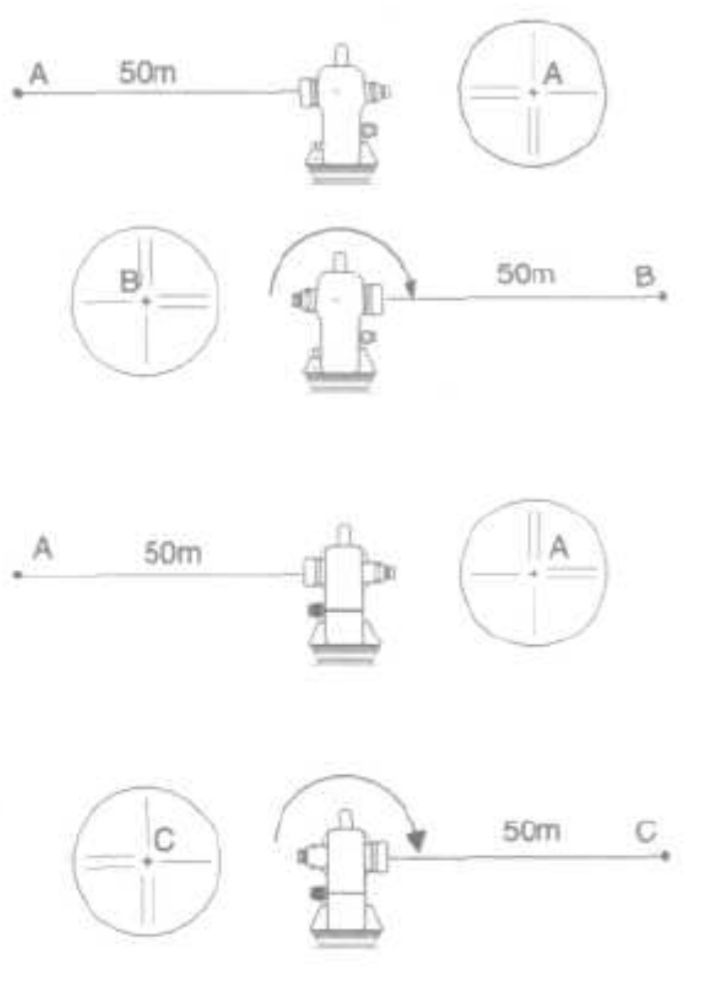
\includegraphics[scale=0.45]{photo1625172362.jpeg} }\\
    Рисунок 1 $-$ \textit{«Коллимация инструмента»}  
\end{center}
\par \textbf{Результат поверки:} Точки совпадают.
\par\textbf{Вывод:} Поверка выполняется.
\par \textbf{Юстировка:} Отвинтите крышку покрывающую 4 регулировочные винты сетки нитей. Регулировочных винта сетки нитей поворачивая крышку против часовой стрелки
\par Определите точку D между В и С т.о. чтобы расстояние CD равнялось ¼ расстояния ВС. (несовпадение ВС в 4 раза больше реальной ошибки за коллимацию из-за того что телескоп при проверке поворачивался 2 раза.
\par Поворачивая регулировочные воротки в верхней, нижней, левой и правой части
окуляра передвиньте вертикальную нить сетки нитей т.о. чтобы она совпадала с точкой
D. По окончании регулировки повторите процедуру проверки. 
\par Если точки В и С совпадают, то дальнейшей регулировки не требуется. В противном случае повторите
регулировку.
\par\textbf{5. Поверка лазерного отвеса.}
\par \textbf{Главное условие:} Вертикальная ось теодолита должна находиться над
точкой центрирования когда лазерный визир будет попадать на точку центрирования.
\par \textbf{Выполнение поверки:} Установите инструмент на штатив на высоту около 1.5м и отгоризонтируйте его. Включите лазерный отвес и заметьте первоначальное расположение лазерного визира на
земле.
\par Поверните инструмент на 180˚ вокруг вертикальной оси и проверьте точку на
земле. Если первоначальная точка центрирования остаётся в пределах 1мм от
первоначального положения визира регулировки не требуется. В противном случае
требуется регулировка состоящая из следующих процедур.
\par \textbf{Результат поверки:} Точка центрирования остаётся в пределах 1мм от
первоначального положения визира.
\par\textbf{Вывод:} Поверка выполняется.
\par \textbf{Юстировка:} Отвинтите крышку регулировочной части окуляра отвеса. Под ней находятся 4
регулировочных винта воротков. Отрегулируйте положение воротков окуляра с
помощью шпильки из набора аксессуаров т. о. чтобы передвинуть
первоначальную точку центрирования к лазерному визиру на ½ величины её
отклонения от визира.
\par Поверните инструмент на 180˚ вокруг вертикальной оси и проверьте точку на
земле. Если первоначальная точка центрирования остаётся менее 1мм от первоначального
положения визира регулировки не требуется. В противном случае требуется повторение
регулировки.
}
\end{document}
